\documentclass[portrait]{a0poster}
% Note: if package conflicts occur, try importing them before triumfposter
\usepackage{triumfposter}

% for example text in columns
\usepackage{lipsum}
\usepackage{float}
\usepackage{multicol}
\columnsep=60pt % spacing between columns
\columnseprule=0pt % vertical line between columns
\usepackage{amsfonts, amsmath, amsthm, amssymb} % For math fonts, symbols and environments

\usepackage{hyperref}
\usepackage[style=ieee]{biblatex}
\addbibresource{sources.bib}

\title{Conversion Coatings on Non-Ferrous Metals}
  % \veryHuge \\ And I Can Also Have a Subtitle -- Smaller Font Possible \\}

% Single Affiliation
% \author{T.~Author1, T.~Author2, and T.~Author3\\TRIUMF, Vancouver, BC, Canada}

% Multiple Affiliations
\author[1]{Kosta Sergakis}
% \author[2]{V.~Author2}
% \author[1]{T.~Author3}
% \author[1,2]{T.V.~Author4}
\affil[1]{Michigan State University, East Lansing, Michigan}
% \affil[2]{University of Victoria, Victoria, BC, Canada}
\date{\vspace{-5ex}}

\begin{document}
\maketitle
\thispagestyle{empty}
\darkheader

\begin{multicols}{2}
\large

\sectiona{Abstract}
  
  In engineering and manufacturing, non-ferrous metals like aluminum, magnesium, and zinc are praised for their strength-to-weight ratios and electrical conductivity. However, these materials are chemically active and susceptible to environmental degradation, which can lead to premature failure or loss of mechanical integrity. To ensure long-term durability, industries rely on conversion coatings - thin layers formed by chemical or electrochemical reactions that transform the metal surface into an adherent, insoluble compound. These coatings serve as a critical foundation, providing corrosion resistance and a superior "key" for subsequent paints, sealants, or adhesives.

\sectionb{The Five Primary Conversion Coatings}

  Chromate Conversion Coatings (CCC) have long served as the benchmark for aerospace and defense due to their unique "active defense" mechanism \hyperref[ccc_diagram]{[Figure 1]}. These coatings contain hexavalent chromium [Cr(VI)] species that remain partly soluble within the film; if the surface is damaged, these ions physically migrate to the scratch to repassivate the exposed metal. While this self-healing capability inhibits both anodic and cathodic corrosion reactions effectively, the high toxicity and carcinogenicity of Cr(VI) have forced a significant industrial shift toward trivalent chromium [Cr(III)] and completely chrome-free alternatives.

  \vspace{0.75cm}

  Anodizing offers a different approach by using an electrochemical process to grow a thick, integrated layer of aluminum oxide directly from the substrate \hyperref[anodizing_diagram]{[Figure 2]}. Unlike a painted-on coating, this oxide layer is structurally part of the metal and cannot chip or peel. The process creates a highly ordered, porous structure that is ideal for absorbing dyes for aesthetic finishes, though these pores must eventually by "sealed" - often in hot water - to close the surface and maximize its corrosion resistance \autocite{asm_surface_2007}.

  \vspace{0.75cm}

  For high-volume industries like automotive manufacturing, Zirconium and Titanium Nano-Ceramics have emerged as the leading eco-friendly replacements for traditional toxic pretreatments. These systems operate at room temperature and form ultra-thin inorganic films, typically only 20 to 100 nanometers thick, through the hydrolysis of oxyfluoride species \hyperref[nano]{[Figure 3]}. Their primary advantage lies in their environmental efficiency, as they produce significantly less hazardous sludge and require less energy than legacy chemical lines.

  \vspace{0.75cm}

  In applications requiring complex material joining, Silane-Based Treatments function as molecular coupling agents that bridge the gap between inorganic metals and organic topcoats like epoxy \autocite{narayanan_surface_2015}. The bonding mechanism is dual-functional: silanol groups form strong covalent Si-O-metal bonds with the substrate, while organic functional groups cross-link directly into the resin of the adhesive or paint.

  \vspace{0.75cm}

  Finally, Phosphate Conversion Coatings remain a staple for steel and multi-metal pretreatment lines. By chemically converting the surface into a polycrystalline layer of zinc, manganese, or iron phosphate, the process creates a high-surface-area "key" that dramatically improves paint adhesion. Beyond simple corrosion protection, specific variants like manganese phosphate are used on high-friction engine components, such as gears and bearings, to provide essential wear resistance and lubricity during the initial "break-in" period of the machinery.

\sectionb{Figures}

  \begin{center}
    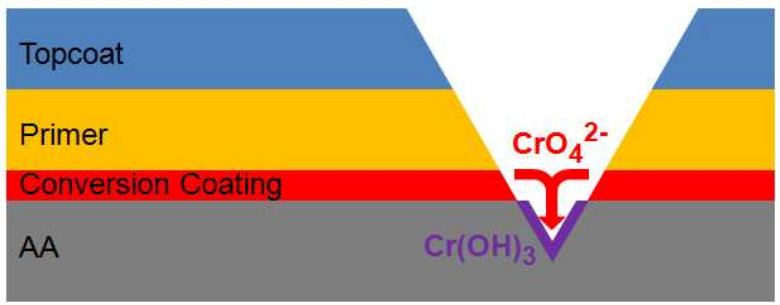
\includegraphics[width=0.42\textwidth]{resources/ccc_diagram.png}
    \\
    \textbf{Figure 1: CCC Diagram} \autocite{li_liangliang_corrosion_nodate}
    \label{ccc_diagram}
  \end{center} 

  \begin{center}
    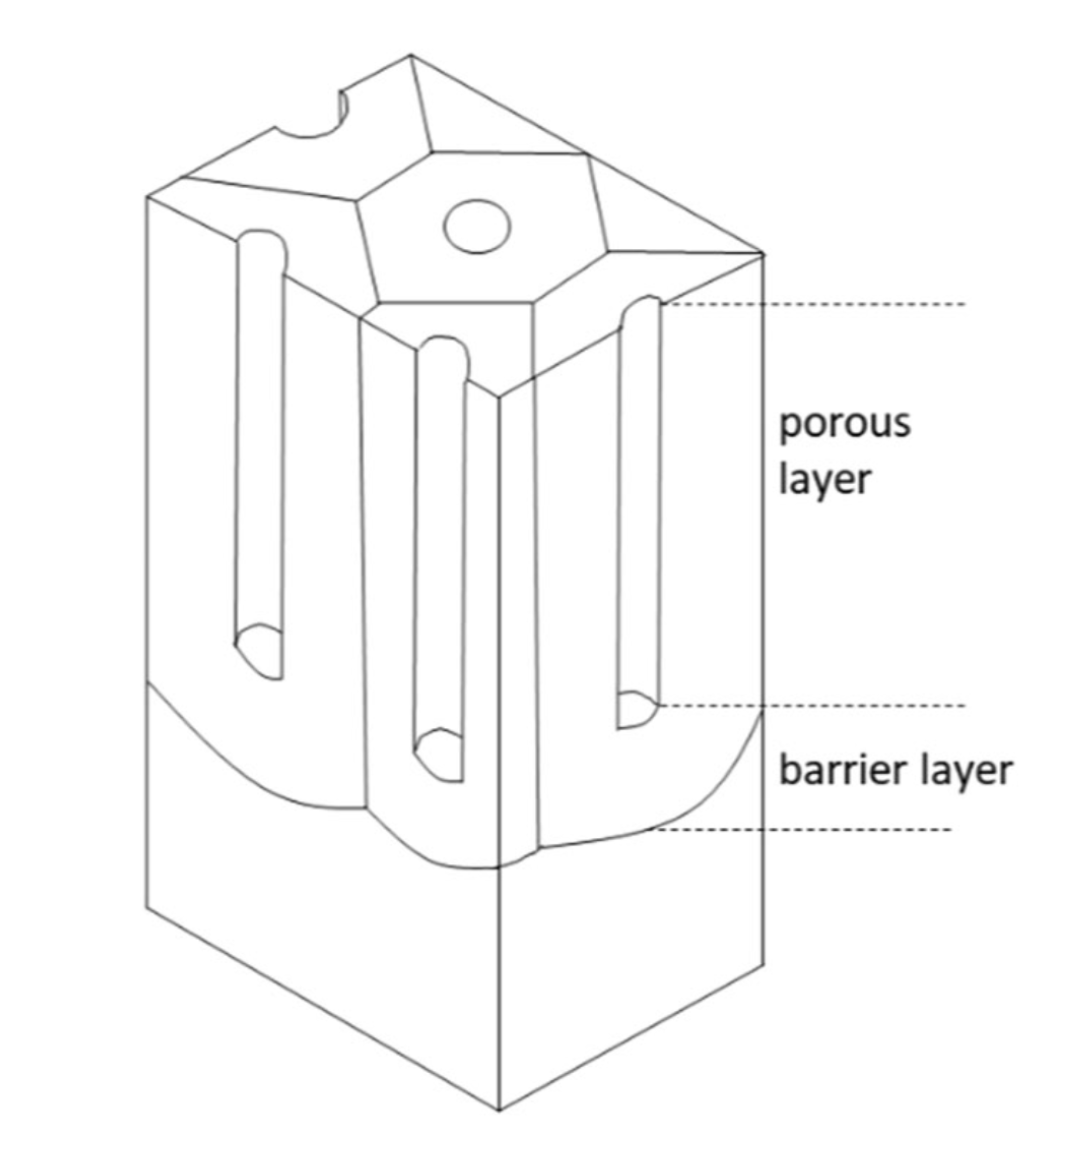
\includegraphics[width=0.3\textwidth]{resources/anodizing_layer_on_aluminum.png}
    \\
    \textbf{Figure 2: Anodizing Layer on Aluminum} \autocite{schneider_anodizingpore_2022}
    \label{anodizing_diagram}
  \end{center}

  % \begin{center}
  %   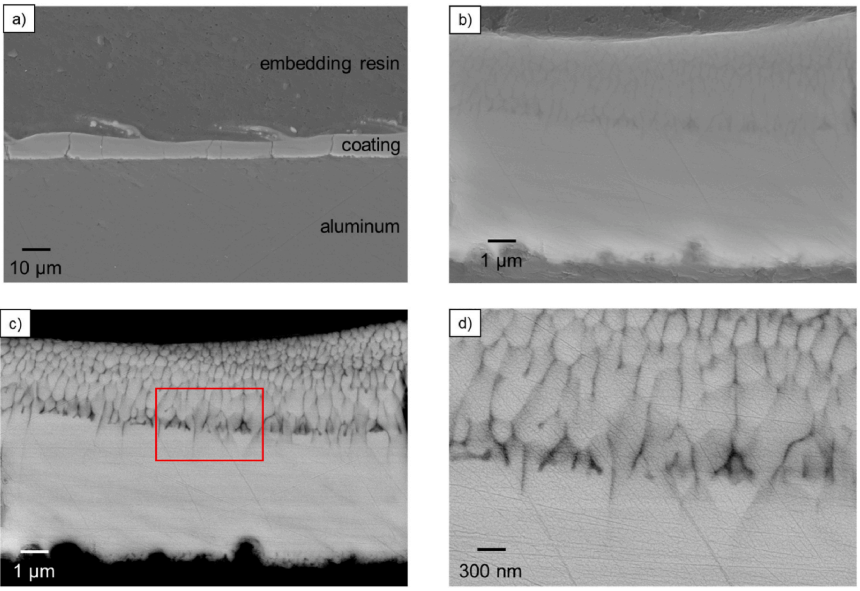
\includegraphics[width=0.3\textwidth]{resources/ceramic_coating.png}
  %   \\
  %   \textbf{Figure X: Anodizing Layer on Aluminum} \autocite{horcher_advanced_2022}
  %   \label{ceramic_coating}
  % \end{center}

  \begin{center}
    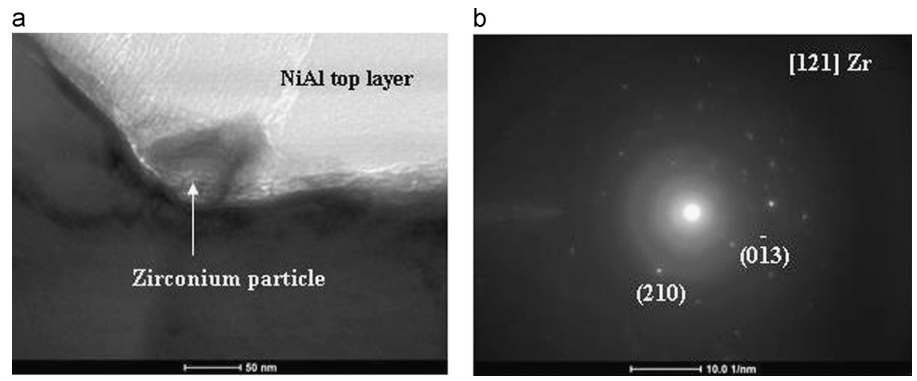
\includegraphics[width=0.46\textwidth]{resources/nanoparticle.png}
    \\
    \textbf{Figure 3: TEM of Zr Nanoparticles in Nickel Substrate} \autocite{zagula-yavorska_nanoparticles_2015}
    \label{nano}
  \end{center}


\sectionb{Conclusion}
\large

  The selection of a conversion coating is a balance between required performance, environmental compliance, and manufacturing efficiency. While hexavalent chromate remains the unmatched standard for self-healing and structural reliability in aerospace, the global push toward sustainability is rapidly elevating the role of nano-ceramics and silane hybrids. Ultimately, whether through the electrochemical growth of an anodized layer or the molecular bridging of a silane treatment, these conversion processes are the indispensable link that allows non-ferrous metals to survive and thrive in the world's most demanding environments.

\sectionb{Acknowledgement}
\small
\printbibliography[]

\end{multicols}

\end{document}